% Schematic of the reduction J(Phi) (Section 2) for a small balanced role-separated instance.
% Variables are vertices of J (U left, W right). Each equation e is a fresh copy of the gadget I_{t_e}
% (rounded box; its new auxiliary vertices inside), whose primaries p_1,p_2,p_3 are identified with
% u_e,w_e,w'_e (the three legs). All copies share g_0,...,g_{k-1} (dashed bus, drawn behind the boxes).
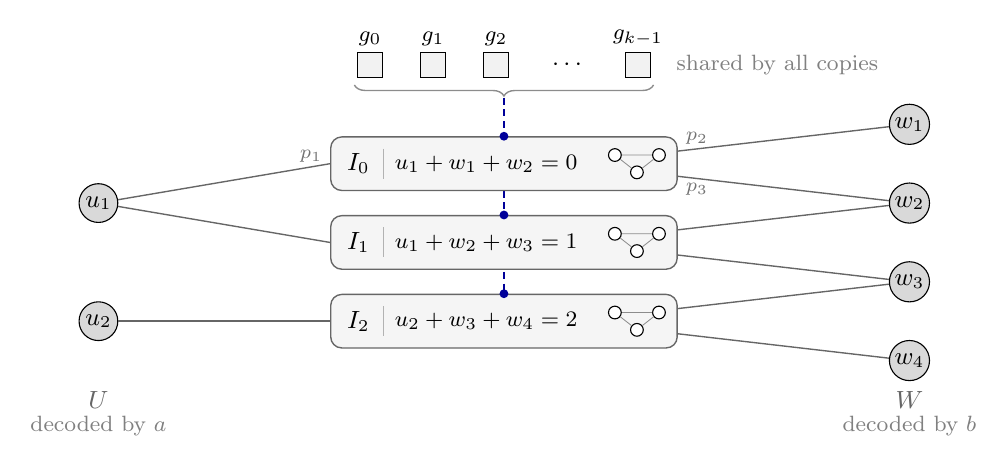
\begin{tikzpicture}[x=1cm,y=1cm,
  prim/.style={circle,draw,fill=black!15,inner sep=1pt,minimum size=14pt,font=\small},
  aux/.style={circle,draw,fill=white,inner sep=0pt,minimum size=4.6pt,line width=0.4pt},
  univ/.style={rectangle,draw,fill=black!5,inner sep=0pt,minimum size=9pt},
  gad/.style={draw=black!60,fill=black!4,rounded corners=4pt,line width=0.5pt,
              minimum width=4.4cm,minimum height=0.68cm,inner sep=0pt},
  leg/.style={line width=0.5pt,black!60},
  glob/.style={dash pattern=on 2.6pt off 1.6pt,blue!60!black,line width=0.7pt},
  tap/.style={circle,fill=blue!60!black,inner sep=0pt,minimum size=3.2pt},
  gname/.style={font=\small,inner sep=1pt},
  eqn/.style={font=\footnotesize,inner sep=1pt,anchor=west},
  plab/.style={font=\scriptsize,text=black!55,inner sep=1.5pt},
  clab/.style={font=\small,text=black!60,inner sep=1pt},
  dlab/.style={font=\footnotesize,text=black!50,inner sep=1pt}]
\def\xu{0}\def\xw{10.3}\def\bx{5.15}% U column, W column, centre of the gadget copies
% ---------------------------------------------------------------- global vertices (shared)
\foreach \n/\x/\l in {0/3.45/g_0, 1/4.25/g_1, 2/5.05/g_2, 3/6.85/g_{k-1}}{
  \node[univ] (g\n) at (\x,4.85) {};
  \node[font=\footnotesize,inner sep=1pt,anchor=south] at ([yshift=1pt]g\n.north) {$\l$};}
\node[font=\small] at (5.95,4.85) {$\cdots$};
\draw[decorate,decoration={brace,mirror,amplitude=4pt},black!45,line width=0.5pt]
  (3.25,4.6) -- (7.05,4.6);
\node[dlab,anchor=west] at (7.3,4.85) {shared by all copies};
% ---------------------------------------------------------------- dashed bus to every copy (behind boxes)
\draw[glob] (\bx,4.44) -- (\bx,1.6);
% ---------------------------------------------------------------- variables (one vertex each)
\node[prim] (u1) at (\xu,3.1) {$u_1$};
\node[prim] (u2) at (\xu,1.6) {$u_2$};
\node[prim] (w1) at (\xw,4.1) {$w_1$};
\node[prim] (w2) at (\xw,3.1) {$w_2$};
\node[prim] (w3) at (\xw,2.1) {$w_3$};
\node[prim] (w4) at (\xw,1.1) {$w_4$};
% ---------------------------------------------------------------- gadget copies
\foreach \n/\y/\t/\eq in {0/3.6/0/{u_1+w_1+w_2=0}, 1/2.6/1/{u_1+w_2+w_3=1}, 2/1.6/2/{u_2+w_3+w_4=2}}{
  \node[gad] (B\n) at (\bx,\y) {};
  \node[gname] at ([xshift=0.36cm]B\n.west) {$I_{\t}$};
  \draw[black!30,line width=0.4pt]
    ([xshift=0.68cm,yshift=0.19cm]B\n.west) -- ([xshift=0.68cm,yshift=-0.19cm]B\n.west);
  \node[eqn] at ([xshift=0.78cm]B\n.west) {$\eq$};
  \node[aux] (x\n a) at ([xshift=-0.80cm,yshift=0.11cm]B\n.east) {};
  \node[aux] (x\n b) at ([xshift=-0.52cm,yshift=-0.11cm]B\n.east) {};
  \node[aux] (x\n c) at ([xshift=-0.24cm,yshift=0.11cm]B\n.east) {};
  \draw[black!45,line width=0.3pt] (x\n a) -- (x\n b) -- (x\n c) -- (x\n a);
  \node[tap] at (B\n.north) {};}
% ---------------------------------------------------------------- legs: p_1 to U, p_2 and p_3 to W
\draw[leg] (B0.west) -- node[plab,pos=0.09,above] {$p_1$} (u1);
\draw[leg] (B1.west) -- (u1);
\draw[leg] (B2.west) -- (u2);
\draw[leg] ([yshift=0.16cm]B0.east) -- node[plab,pos=0.09,above] {$p_2$} (w1);
\draw[leg] ([yshift=-0.16cm]B0.east) -- node[plab,pos=0.09,below] {$p_3$} (w2);
\draw[leg] ([yshift=0.16cm]B1.east) -- (w2);
\draw[leg] ([yshift=-0.16cm]B1.east) -- (w3);
\draw[leg] ([yshift=0.16cm]B2.east) -- (w3);
\draw[leg] ([yshift=-0.16cm]B2.east) -- (w4);
% ---------------------------------------------------------------- column labels
\node[clab] at (\xu,0.6) {$U$};
\node[dlab] at (\xu,0.27) {decoded by $a$};
\node[clab] at (\xw,0.6) {$W$};
\node[dlab] at (\xw,0.27) {decoded by $b$};
\end{tikzpicture}
